\documentclass[a4paper]{article}

\usepackage{sectsty}
\usepackage{graphicx}
\usepackage{hyperref}

\sectionfont{\fontsize{12}{15}\selectfont}

\title{Scientific Software / Technisch-wetenschappelijke software: Assignment 1}
\author{Pavel Mačák}

\begin{document}

\maketitle

Number of hours spent: 33

\section{How did you design your code? Explain how you split functionality across modules/subroutines/functions. Why?}
Code is split to five different files - four modules and one main file. The following list goes in order of dependencies.

\begin{itemize}
	\item \textit{siqrd\_settings.f90}
	\item \textit{io\_module.f90}
	\item \textit{methods\_module.f90}
	\item \textit{simulation\_module.f90}
	\item \textit{siqrd.f90}
\end{itemize}

\subsection{Settings module}
	In this module various parameters known at compile time are set. Namely the working precission of floating point numbers, name of input file (by default \textit{parameters.in}), time horizon of the simulation $ T $ and number of steps $ N $. Stopping criteria of Newton's method are also included. This means that all customisable settings of the program are in one place and are thus comfortable to adjust.
	
\subsection{I/0 module}
	This module defines subroutines used for specific input and formatted output. Getter functions for input parameters ($ \beta,\,\mu,\,\gamma $ etc.) and application specific variables (\textit{SIQRD}) are included because this is also related to format of input/output data.
	
\subsection{Methods module}
	Here, the three required methods are implemented in a very general way, so they could be easily reused for other applications. Module also defines application dependent functions evaluating $ SIQRD $ equations (\textit{fS, fI, fR} etc.) and also derivatives of these functions (\textit{dSdS, dSdI, dSdR} etc.) needed for Jacobian in Euler's backward method.
	
	The three subroutines corresponding to three methods of solution, could still be more generalized if function \textit{fvals}, which in this case evaluated the $ SIQRD $ equations, would be passed as one of the arguments. This was not implemented in this case, because the Euler's backward subroutine would also need the Jacobian function as argument, which would in turn mean a different interface from the other two methods. 
	
\subsection{Simulation module}
	This module controls the flow of the simulation. The main subroutine is \textit{simulateSIQRD}, defined as follows.
	\begin{verbatim}
	subroutine simulateSIQRD(method, methodName, simulationParameters, outputFileName)
	    character(*), intent(in) :: methodName
	    real(wp), dimension(:), intent(in) :: simulationParameters
	    character(*), optional, intent(in) :: outputFileName
	\end{verbatim}
	Method is an external subroutine with this interface.
	\begin{verbatim}
	subroutine method(vars, parameters)
	    real, dimension(:,:), intent(inout) :: vars
	    real, dimension(:), intent(in) :: parameters    
	\end{verbatim}
	This corresponds to interface of subroutines \textit{eulerForward, heunMethod} and \textit{eulerBackward} defined in the Methods module. The method should calculate values in the next time step and put these to the last column of matrix \textit{vars}.
	Second argument is a custom naming of the method which will appear at the beginning of the output file name, as required by assignment. Third argument is vector of simulation parameters. This has the $ \delta t $ parameter as first element and the rest are the inputs from \textit{parameters.in}. Last argument is optional \textit{outputFileName}, which overrides the default naming convention of \textit{.out} file.
	
	The main loop is preceded by data definitions and initialisation, whose format is further discussed in section \ref{sec:data}. The loop itself is fairly simple and well commented in the source code. 
	
\subsection{Siqrd main program}
	The source for program SIQRD is in the file \textit{siqrd.f90}. The program firstly reads parameters from \textit{parameters.in} using \textit{readParams} subroutine from I/O module and then runs the simulation using different methods.

\section{How did you store the data and parameters?} \label{sec:data}
\subsection{Parameters}
Parameters that are read from input file \textit{parameters.in} are stored in one dimensional array. This array also contains the $ \delta t $ parameter in the first position, which is than followed by parameters $ \beta, \, \mu, \, \gamma, \, \alpha, \, \delta, \, S_0 $ and $ I_0 $. Nevertheless remembering this exact order (and number) is of less importance because the getter functions are used to access these parameters.

Simulation parameters that are known at compile time and are thus constant are defined in Settings module. These include input file name, number of time steps, final time of calculation and Newton's method settings.

It should be noted that parameter $ \delta t $ is also known at compile time, but it is stored in the array together with input parameters. It was done this way, so that $ \delta t $ could be changed during the simulation and thus allow for easier implementation of dynamic time stepping if later desired.

\subsection{Data}
The structure of data is defined in Simulation module. The variables $ S,\,I,\,Q,\,R$ and $D $ are stored in a two dimensional array. Bearing in mind the column mayor storage of arrays used in fortran, rows represent the $ SIQRD $ variables and columns are the different time layers. All three methods only require variables from one previous time layer, so the variables array in this case is of dimension 5x2. The methods than work with last two columns of the array, considering the penultimate column as previous time layer and writing the data for new time step in the last column.

\section{How do you set the precision of the floating point numbers? Why?}
The precision is set in Settings module using the parameter \textit{wp} (working precission). By default this is set to single precision, as was required in the \textit{Assignment.pdf}.


\section{Which stopping criteria did you choose for Newton's method? Why?}
The Newton's method stops either when reaching maximum amount of iteration or when the backward error is sufficiently small. For $ ||G(x^{(s)}_{k+1})|| $ the chosen norm is the maximum norm $ ||x||_{\infty} $. The desired size of backward error can also be set. When the specified precision is not reached, the program aborts the simulation with an error message. This behaviour can also be turned off in Settings module. These stopping criteria are used because they are easy to implement, but also provide good control of the algorithm. The forward error on the other hand seems more viable in terms, that it actually checks the difference in values of variables $ x_i $, which we are mainly interested in. But also there has to be the step of checking whether the equation $ G(x_i)=0 $ is satisfied, so one could say that the forward error checking adds an additional criterion in comparison to the backward error, but requires the solver to remember values of $ x_n, \, x_{n+1}^{(s)} $ and $ x_{n+1}^{(s+1)} $ in contrast to backward error, which does not need $ x_{n+1}^{(s)} $ for convergence evaluation.
Of course  $ x_{n+1}^{(s+1)} $ has to satisfy the equation $ G(x_{n+1}^{(s+1)})=0 $ well enough to be consider as $ x_{n+1}^{*} $ in the forward error formula.

\section{What do you observe when you run your first program on different compilers? Can you explain what happens based on the IEEE 754 format?}
The implementation of the first program gives same results for all three compilers. The only difference is when switching the format of floating point numbers. The result in double precision and single precision floating point numbers differs in the last digit when rounded to nearest integer. The question kind of implies that something more remarkable should happen, but this is all that I observed.

The reason could be that the term $ (1+r)^d $ is a relatively big number in comparison to $ I_0 $, which could lead to different multiplication error for each precisions. Also the term $ (1+r)^d $ is probably computed as approximation of logarithmic and exponential function and the precision of the implementation could differ for double and single precision floats.


\section{How do you ensure your implementation is correct?}
Firstly it was ensured that the implementation works for the most basic cases, with all parameters set to zero, then enabling some parameters etc. Then stability of the solution with respect to $ \delta t $ step size and other calculation parameters was briefly investigated to get an idea of their appropriate settings. It was discovered that the stability is very dependant of the parameter $ \beta $ (or basically the largest parameter, but it makes sense that the $ \beta $ would be largest in many cases). Also it is good to check the sum of $ SIQRD $ variables, which should be constant at all times and thus equal to the initial population $ S_0 + I_0 $. Furthermore, one could impose restrictions on each variable in sense that, none should be negative or grow above the initial population count. The latest was also implemented in the Simulation module by subroutine \textit{restrict}.

Then two model cases for which the results are known have been simulated.

\newpage
\subsection{First test case}
Another verification was then performed by comparing the implemented $ SIQRD $ model to a model case of $ SIQ $ model, that can be found on \href{https://www.maa.org/press/periodicals/loci/joma/the-sir-model-for-spread-of-disease-the-differential-equation-model}{Mathematical Association of America webpage}. The initial conditions and parameters were set accordingly to correspond to the $ SIQ $ model as follows
\begin{equation}\label{eq:parameters}
\beta = 0.5;\,\,
\gamma = 0.33;\,\,
\mu=\,\alpha=\,\delta = 0;\,\,
S_0 = 1;\,\,
I_0 = 1.27 \cdot 10^{-6}.\,\,
\end{equation}
The results correspond very well as can be seen from Figures  \ref{fig:siqfrominternet}, \ref{fig:eulerbackwardsircomparisson}, \ref{fig:eulerforwardsircomparisson} and \ref{fig:heunsircomparisson}. The peak of infected people happens between 70th and 80th day with value roughly below $ 10 \%$ of the original population.


\begin{figure}[h]
	\centering
	\begin{minipage}{.48\textwidth}
		\centering
		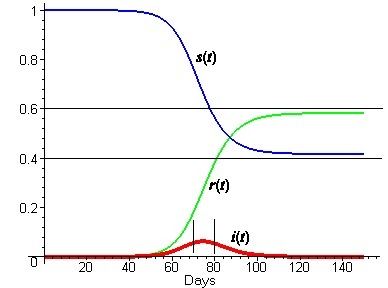
\includegraphics[width=1\linewidth]{figs/sir.jpg}
		\caption[Model case]{Model SIR case results from MAA webpage (added black leading lines for better comparison)}
		\label{fig:siqfrominternet}
	\end{minipage}%
	\begin{minipage}{.52\textwidth}
		\centering
		\includegraphics[width=1\linewidth]{figs/eulerBackward_sir_comparisson}
		\caption[Backward SIR]{Model SIR case simulated with Euler's backward method}
		\label{fig:eulerbackwardsircomparisson}
	\end{minipage}
\end{figure}
  
\begin{figure}[h]
	\centering
	\begin{minipage}{.5\textwidth}
		\centering
		\includegraphics[width=1\linewidth]{figs/eulerForward_sir_comparisson}
		\caption[Forward SIR]{Model SIR case simulated using Euler's forward method}
		\label{fig:eulerforwardsircomparisson}
	\end{minipage}%
	\begin{minipage}{.5\textwidth}
		\centering
		\includegraphics[width=1\linewidth]{figs/heun_sir_comparisson}
		\caption[Heun SIR]{Model SIR case simulated using Heun's mehod}
		\label{fig:heunsircomparisson}
	\end{minipage}
\end{figure}

\subsection{Second test case}
Second test case comes from article  \href{https://www.ncbi.nlm.nih.gov/pmc/articles/PMC5963332/}{Mathematical models of SIR disease spread with combined non-sexual and sexual transmission routes}. The parameters for this calculation are
\begin{equation}\label{eq:parameters2ndExample}
\beta = 10;\,\,
\gamma = 1;\,\,
\mu=\,\alpha=\,\delta = 0;\,\,
S_0 = 0.95;\,\,
I_0 = 0.05.\,\,
\end{equation}
Corresponding figures are \ref{fig:siqfrominternetMiller}, \ref{fig:eulerbackwardsircomparissonMiller}, \ref{fig:eulerforwardsircomparissonMiller} and \ref{fig:heunsircomparissonMiller}. Again there is a very good agreement between this implementation and the test case. A note on the side, this particular test case helped me to discover a bug in both of my Heun's method and Euler's backward method implementation.

\begin{figure}[h]
	\centering
	\begin{minipage}{.5\textwidth}
		\centering
		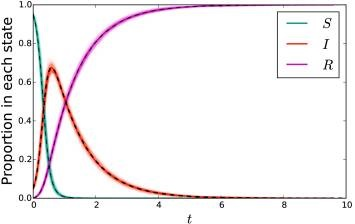
\includegraphics[width=1\linewidth]{figs/sirMiller.jpg}
		\caption[Model case2]{Second model SIR case results from J. C. Miller's article}
		\label{fig:siqfrominternetMiller}
	\end{minipage}%
	\begin{minipage}{.5\textwidth}
		\centering
		\includegraphics[width=1\linewidth]{figs/eulerBackward_sir_comparisson_Miller}
		\caption[Backward SIR2]{Second model SIR case simulated using Euler's backward method}
		\label{fig:eulerbackwardsircomparissonMiller}
	\end{minipage}
\end{figure}

\begin{figure}[h]
	\centering
	\begin{minipage}{.5\textwidth}
		\centering
		\includegraphics[width=1\linewidth]{figs/eulerForward_sir_comparisson_Miller}
		\caption[Forward SIR2]{Second model SIR case simulated using Euler's forward method}
		\label{fig:eulerforwardsircomparissonMiller}
	\end{minipage}%
	\begin{minipage}{.5\textwidth}
		\centering
		\includegraphics[width=1\linewidth]{figs/heun_sir_comparisson_Miller}
		\caption[Heun SIR2]{Second model SIR case simulated with Heun's mehod}
		\label{fig:heunsircomparissonMiller}
	\end{minipage}
\end{figure}

It is also important that the methods came to an agreement with any other tested "reasonable" combination of parameters, which also included the variables $ Q $ and $ D $.

Furthermore, it could be interesting to find out the parameters values for which the population is in danger of extermination due to the disease. From a few experiments it became obvious that the immunity loss coefficient plays a mayor role in this. This could be interpreted as if the disease mutates violently (cured people won't be immune to the mutated disease) while retaining it's capability to kill people, it would very probably lead to an apocalyptic scenario. 


\section{What do you see when you compare the three methods implemented for simulating the SIQRD model?}

As the Heun's method is of higher order of accuracy, it can capture steeper changes better with the same grid step in comparison to both Eulers' methods. This can be also demostrated for example by comparing the end results of all the methods, while decreasing the step size $ \delta t $. For coarse time stepping, all three results can be slightly different (but all already "make sense") as for the model case shown in Figure \ref{fig:assignmentspecial}. By refining the grid they all come to agreement in the end. And as expected, the Heun's method converges the fastest to such value. It also seems from Figure \ref{fig:assignmentspecial} that Heun's method is much better at capturing quick changes in function values.

\begin{figure}[h]
	\makebox[\textwidth][c]{\includegraphics[width=1.4\linewidth]{figs/assignment_special}}
	\caption[Assignment case]{Results of all three methods with parameters $ \beta = \gamma = 10.0;\,\, \alpha = 1.0;\,\, \mu=\,\delta = 0;\,\, S_0 = 100;\,\, I_0 = 5;\,\, N = 150;\,\, T = 30. $}
	\label{fig:assignmentspecial}
\end{figure}


The other question is stability of selected methods. The Euler's backward method is implicitly stable (which in practice does not hold infinitely due to finite precision of the computations) and thus beats both remaining methods in this way. It pays a high price for this, which is solving a system of linear equations many times in each iteration. But in some cases (like simulations with very high time horizon) the implicit stability could outweigh this, because then a much bigger time step can be selected in order to get fast estimation of the results, which in turn could be used to select a correct (or even dynamic) time step value for the more accurate Heun's scheme.

In terms of implementation difficulty, the Heun's method and Euler's forward are more or less the same. Although Heun's method requires two evaluations of $ \textbf{f}(\textbf{x}) $, but that makes little difference in terms of coding. Euler's backward method requires a lot more work. Firstly to analytically derive the Jacobian and then implement it correctly takes some time, but that is the price for stability. 

To sum it up, from my point of view the Heun's method beats the Euler's forward method. Only for the case that evaluation of function $ \textbf{f}(\textbf{x}) $ is really time consuming, the Euler's forward method could be of use for a fast first simulation. As stated previously, the Euler's backward method excels in stability for a price of higher computational cost.






\end{document}